\newpage
\section{Resultate}

\noindent\begin{minipage}[t]{0.5\textwidth}
\vspace{0pt}
    \begin{figure}[H]
    	\centering
    	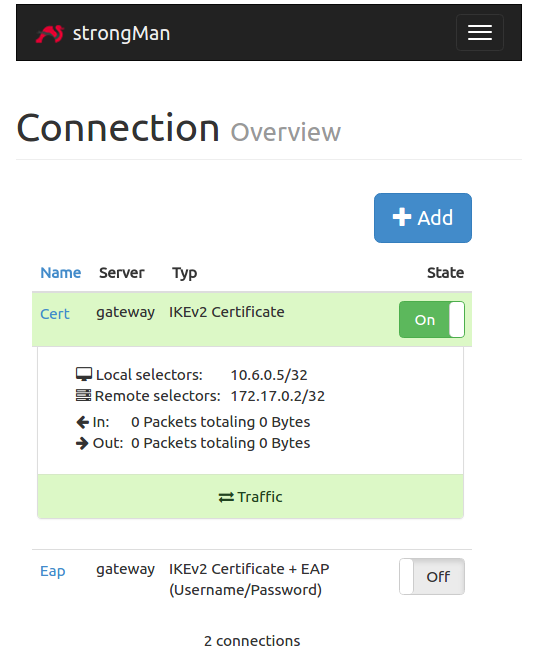
\includegraphics[width=230pt]{images/con_overview.png}
    	\caption{Connection Overview}
    \end{figure}
\end{minipage}
\hfill
\begin{minipage}[t]{0.5\textwidth}
\vspace{0pt}
\subsection{Management-Oberfläche für VPN Clients}
Die Management-Oberfläche der strongMan Applikation gibt eine Übersicht über alle erfassten Verbindungen. Diese können per Klick auf den Namen geändert oder gelöscht werden.\\
Zum Starten oder Stoppen der konfigurierten VPN Verbindungen ist der Toggle Button gedacht.\\
Wurde ein VPN-Tunnel erfolgreich aufgebaut, werden Statusinformationen angezeigt.
\end{minipage}
\medskip


\noindent\begin{minipage}[t]{0.5\textwidth}
\vspace{0pt}
\subsection{Zertifikatsverwaltung}
Unter dem Reiter Certificates finde sich ein Zusammenstellung aller selbst erfassten Zertifikate und derer die von strongSwan verwaltet werden. Diese werden über die Vici-Schnittstelle geladen und auch in der Datenbank persisitiert. Es ist möglich nach Zertifikaten zu suche, diese zu sortieren und durch das Auswählen weitere Information anzuzeigen.
\end{minipage}
\hfill
\begin{minipage}[t]{0.5\textwidth}
\vspace{0pt}
    \begin{figure}[H]
    	\centering
    	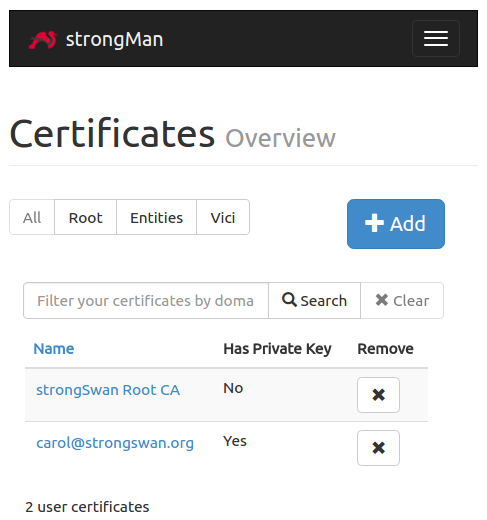
\includegraphics[width=230pt]{images/certificate_overview.png}
    	\caption{Certificate Overview}
    \end{figure}
\end{minipage}
\newpage

\subsection{Ausblick}
strongMan implementiert nach Abschluss dieses Projekts Clientfunktionalitäten wie oben beschrieben. Ausbaumöglichkeiten gibt es in der nicht realisierten Kann Anforderung der Serverfunktionalität. Mit dieser Erweiterung soll es möglich sein, einen VPN Gateway zu konfigurieren und auch zu verwalten. Gerade die Verwaltung eines Gateways zieht aufwändigere Funktionalität bezüglich Security Associations Management, Visualiserung der Verbindungen, sowie Statistikinformationen mit sich.\\ 


Wenn gewünscht kann das Benutzermanagement von derzeit einem Standardbenutzer auf eine belibige Anzahl ausgebaut werden. Diese Änderung ermöglicht die getrennte Verwaltung von Verbindungen in einem Multiusersystem.

Weiter ist derzeit strongMan auf wenigen Unix Distributionen lauffähig. Es können weitere Distributionen getestet und eine Portierung auf Windows versucht werden.


\subsection{Auswertung}
\begin{table}[H]
	\centering
    \begin{tabular}{|p{0.5\textwidth}|p{0.5\textwidth}|}
    \hline    
    \rowcolor{lightblue}
	Ziel &  Bemerkung\\ \hline   
	Implementation einer grafischen Management-Oberfläche mit Django für strongSwan
    zur Konfiguration eines VPN Clients für folgende vier IKEv2 Authentisierungsmetho-
    den:
    \begin{enumerate}
        \item X.509 Zertifikat und privater RSA/ECDSA Schlüssel
        \item EAP mit Benutzername/Passwort
        \item Zweirunden-Authentisierung mit Methode 1) gefolgt von Methode 2)
        \item EAP-TLS mit X.509 Zertifikat und privatem RSA/ECDSA Schlüssel
    \end{enumerate}
	& Die definierten Authentisierungsmethoden werden unterstützt und durch die Architektur der strongMan Applikation sind Erweiterungen möglich.  \\ \hline
	Oberfläche zur Verwaltung von X.509 End Entity und CA Zertifikaten, sowie privater
    RSA/ECDSA Schlüssel. & strongMan ermöglicht das Hinzufügen und Entfernen von Zertifikaten,  weiter ist das Filtern und Suchen möglich. Als zusätzliches Feature kann einem Zertifikat ein Nickname gesetzt werden, bei der Identifikation hilft.
    \\ \hline
    Persistierung der Konfigurationsdaten in einer Datenbank. & Alle Konfigurationsdaten, sowie Zertifikate werden in der Datenbank gespeichert. Dabei wird standardmässig eine SQLite Datenbank verwendet, welche es ermöglicht ohne zusätzliche Konfiguration und Installation die Applikation zu verwenden. \\ \hline
    Verschlüsselte Ablage der RSA/ECDSA Authentisierungsschlüssel in der Datenbank. & Die schützenswerten Daten Privatekeys und strongSwan Secrets (Bsp. EAP Passwort) werden durch eine AES256 Verschlüsselung in der Datenbank persistiert. \\ \hline
    Starten und Stoppen von konfigurierten VPN Verbindungen & Korrekt erfasste Verbindungen können über die Vici-Schnittstelle gestartet und gestopppt werden. \\ \hline
    Darstellung von Statusinformation über aktive VPN Verbindungen & Informationen zu Local- und Remoteselectors, Traffic sowie Logs werden dargestellt. \\ \hline
    \textbf{Optional}: Oberfläche zur Konfiguration eines VPN Gateways & Die Erweiterung zur Gateway/Server Konfiguration wurde nicht implementiert. Gegen Ende des Projektes wurde entschieden, dass der Fokus auf die Clientseite gesetzt wird und dieser noch verbessert werden soll.   \\ \hline 
    \end{tabular}
    \caption[Auswertung]{Auswertung}
\end{table}
\medskip \medskip